\documentclass[14pt,a4paper, titlepage]{article}
\usepackage{graphicx}
\usepackage{url}
\usepackage{hyperref}
\usepackage{listings}
\usepackage{amsmath}
\usepackage{csquotes}
\newcommand{\ext}[3]{\ensuremath{\&{#1}[#2](#3)}}
\DeclareMathOperator{\leftimpl}{:-}
\setlength{\tabcolsep}{1.5pt}
\lstset{
    literate={~} {$\sim$}{1}
}

\newcounter{examplecounter}
\newenvironment{example}{\begin{quote}%
    \refstepcounter{examplecounter}%
  \textbf{Example \arabic{examplecounter}}%
  \quad
}



\begin{document}
\setcounter{page}{3}
\newcommand{\dlvhex}{{\sc dlvhex}}
\newcommand{\hex}{{\sc hex}}
\setcounter{secnumdepth}{4} % how many sectioning levels to assign numbers to
\setcounter{tocdepth}{4}    % how many sectioning levels to show in ToC

\newtheorem{exmp}{Example}[section]


\begin{titlepage}
    \centering
    \vfill
    
\includegraphics[width=16cm,height=4.5cm,scale=1.5]{biglogo_whitebg}
    \vfill
    {\bfseries\Large
        User Guide
        \vskip4cm
        Mustafa Mehuljic \vskip1cm Christoph Redl
    }    
    
\end{titlepage}

% Abstract part
\begin{abstract}
This document provides a user guide for the Answer Set Programming (ASP) system called \dlvhex{} developed at Vienna University of Technology. ASP is a declarative problem solving paradigm, rooted in logic programming and nonmonotonic reasoning, which has been gaining increasing attention during the last years. The \dlvhex{} system is a reasoner for computing the models of so-called \hex{}-programs, which are an extension of \emph{answer-set programs} towards integration of \emph{external computation sources}. This guide aims at enabling users of this system to interoperate with a broad set of external computation sources. The guide refers to release 2.4.     
\end{abstract}

% Generates table of contents
\tableofcontents
\newpage

\section{Introduction} % Section No.1
The \dlvhex{} system is a logic-programming reasoner for computing the models of so-called \hex{}-programs, which are an extension of \emph{answer-set programs} towards integration of \emph{external computation sources}. To enable access to external information, \hex{}-programs extend programs with external atoms, which allow for a bidirectional communication between the logic program and external sources of computation (e.g. description logic reasoners and Web resources) \cite{extatoms}. The system is developed motivated by the need to interoperate with a broad set of external computation sources and the observation, that for meta-reasoning in the context of the Semantic Web, no adequate support is available in ASP to date. To overcome this, \hex{}-programs have been introduced, which support higher-order logic programs (which accommodate meta-reasoning through higher-order atoms) with external atoms for software interoperability.

This guide helps ASP novices to make use of the system. It provides a reference of the features of the tool that ASP might be tempted to exploit. The language of \hex{}-programs is an extension of disjunctive datalog. It largely implements the ASP-Core-2 Standard \cite{ref} and extends it with external atoms. 


\subsection{Download and Installation}
\dlvhex{} is written in the C++ programming-language and published under the GNU Lesser General Public License \cite{licnc}. In this section we provide an overview of the download and installation process. For a quick overview, some examples and the possibility to evaluate \hex{}-programs directly in the browser, the online demo at \url{http://www.kr.tuwien.ac.at/research/systems/dlvhex/demo.php} is provided. However the system can also be installed locally. 

\subsubsection{Building from source}
There are two possibilities to install \dlvhex{} system from source: install the latest stable release of the system or install the latest development version which may not be stable. Both ways are described in following sections.  

\paragraph{Latest release version (tarball)}
Packages (tarballs) of \dlvhex{} can be downloaded from the project page \url{http://www.kr.tuwien.ac.at/research/systems/dlvhex} The latest release of the software runs on Linux-based systems, Mac OS X and Microsoft Windows. Installation instructions are given in the {\tt INSTALL} and {\tt README} files of the \dlvhex{} and plugin source directories. Changes between versions can be found in the {\tt NEWS} files and in detail in the {\tt ChangeLog} file. 

The system requires the following packages: git, gcc (version 4.8 or later), g++ (version 4.8 or later), BZ2 library, Python (version 2.7 or later), bison, scons, cmake, automake, autoconf, standard C++ library (version 4.8 or later), Curl library (version 4 or later) and libool. Also the Boost library (version 1.55 or later) is required. The latest Boost library version is available at \url{http://www.boost.org/}. After downloading it to the new folder the following steps should be followed in order to properly install it. After extraction, the folwing commands need to be executed:
\\ \centerline{\texttt{./bootstrap.sh}}
\centerline{\texttt{./b2 install --prefix=PREFIX}} In this command \texttt{PREFIX} is the directory where Boost should be installed. After downloading latest release version by executing the following sequence of commands \dlvhex{} will be successfully installed:
\\ \centerline{\texttt{./configure}} To enable the Python features of \dlvhex{}, \texttt{--enable-python} is to be added as option of \texttt{configure}. Afterwards, the following command builds the system:
\\ \centerline{\texttt{make}} To allow using of multiple cores one should specify the \texttt{-jN} option to make use of N cores. Finally the following
\\ \centerline{\texttt{make install}} installs the package in the location specified with configure.  
   
\paragraph{Development version (git clone)}
The source code of \dlvhex{} is hosted on github at \url{https://github.com/hexhex/}. To get the latest development version it is necessary to git clone system as follows:
\\ \centerline{\texttt{git clone https://github.com/hexhex/core --recursive}} 
After cloning to the desired directory it is necessary to execute bootstrap.sh script from there invoking \\ \centerline{\texttt{./bootstrap.sh}}. 
After cloning and bootstrapping, the steps from Section 1.1.1.1 (\texttt{configure, make} and \texttt{make install}) are to be followed in order to complete installation.
We provide a script which should install \dlvhex{} automatically on your system, which can be found at \url{https://github.com/hexhex/core/blob/master/scripts/setupdlvhex.sh}.
Once installation is completed, the system can be used from the terminal as follows:\\ 
\centerline{\texttt{shell\$ dlvhex2 program.hex}} where \texttt{program.hex} refers to the input program. Various additional options are available and explained in following sections.    

\subsubsection{Pre-built binaries}
We provide pre-built binaries of \dlvhex{} for some systems. For details see our website \url{http://www.kr.tuwien.ac.at/research/systems/dlvhex/index.html}. 

\subsection{Outline}
This guide is organized as follows: Section 2 provides an introductory example which will be used to explain the problem instance, the encoding and its solution. Section 3 is focused on input language of the \dlvhex{}. In Section 4 we introduced three real life problems which can be solved using our system. Section 5 is focused on description of external interfaces which are written in C++ or Python. Input-related warnings and errors are described into more details in Section 6 and finally in Section 7 we describe possible future work that may be considered.

\section{Quickstart} % Section No.2
As an introductory example, we consider a \emph{social graph} as used in social networks. Beginning from a simplified scenario, we stepwise extend it to present various features of \dlvhex{}.

\subsection{Problem Instance}
A \emph{social graph} is a graph that represents interconnections among people, groups 
and organizations in a social network. Services such as Facebook facilitate the exchange 
of information, news, photographs, literary works, music, art, software, opinions or even 
money among users. In this environment, the social graph for a particular user consists 
of the set of nodes and edges which model other users that are directly connected, to that actor. 
Individuals and organizations, called actors, are nodes on the graph. Interdependencies, 
called ties, can be multiple and diverse, including such characteristics or concepts as age, 
gender, race, genealogy, chain of command, ideas, financial transactions, trade relationships, 
political affiliations, club memberships, occupation, education and economic status. 
Social graphs contain edges between one person and related people, places, and things they interact 
with online. For this particular example, we consider a simulation of Facebook social graph. 

Consider the situation where a birthday party should be organized and a specific number of friends will
 be invited. The \emph{person $X$} which organizes the event wants to call his or her friends and friends of these friends up to some distance from the root node $X$. A \emph{depth constraint} specifies how many edges we can go away from the root node $X$.
 

We make use of an external source which returns for a given person all direct friends, while a direct access to the full graph is not available due to privacy issues imposed by social networks. Also, due to the large amount of data, importing the whole graph would be infeasible (billions of users), while only a small fraction is relevant for the application. The external source finds for a person $X$ all neighbour nodes (successor nodes). More details about the external source implementation are given in Section 5. 
               

\subsection{Problem Encoding}
The problem can be modeled as a \hex{}-program as follows:

\begin{exmp}
\begin{align*}
r_1\colon & \mathit{personOfInterest}(\mathit{john}).\\
r_2\colon & \mathit{friendOfDegree}(\mathit{P, 0, P}) \leftimpl  \mathit{personOfInterest}(P).\\
r_{3}\colon \mathit{friendOfDegree}(\mathit{P, DegPlus, F2}) \leftimpl & \mathit{friendsOfDegree}(\mathit{P,Deg,F1)},\\
& \ext{friendsOf}{F1}{F2}, \mathit{DegPlus = Deg + 1}, \mathit{DegPlus < 2},\\
& \mathit{\#int(DegPlus)}, \mathit{\#int(Deg)}.\\
r_{4}\colon & \mathit{invite(P)} \text{ v } \mathit{ninvite(P) \leftimpl  friendOfDegree(john,X,P), \#int(X).}\\
r_{5}\colon & \leftimpl   \mathit{not} \text{ 4 } = \mathit{\#count} \{ P : \mathit{invite(P)} \}.
\end{align*}
\end{exmp}
The rule $r_1$ specifies that the person who organizes the event and initializes the search. 

The rule $r_2$ specifies that initiating person has distance 0 from him or her. The main computational part of the program is the rule $r_3$. The main computational part of the program is the following rule   
\begin{align*}
r_{3}\colon& \mathit{friendOfDegree}(\mathit{P, DegPlus, F2}) \leftimpl \mathit{friendsOfDegree}(\mathit{P,Deg,F1)},\\
& \ext{friendsOf}{F1}{F2}, \mathit{DegPlus = DegPlus + 1}, \mathit{DegPlus < 2},\\
& \mathit{\#int(DegPlus)}, \mathit{\#int(Deg)}.
\end{align*} 
It cyclically queries all  friends of already known persons and increments the distance with each iteration. Variables used in these predicates are: 

\begin{itemize}
\item $F$1 represents the person for which we are looking for the successors.

\item $F2$ is variable which holds successor nodes of $F1$. 

\item $P$ represent person of the interest.

\item $Deg$ and $DegPlus$ are variables used to keep distance from the root node.
\end{itemize}


The external atom \ext{friendsOf}{F1}{F2} has one input and one output parameter. For input $\mathit{F1}$, 
it finds all successor nodes of it and returns them in $\mathit{F2}$. The implementation of the plugin is discussed in Section 5. The atom
\begin{align*}
& \mathit{friendOfDegree(P, Deg, F1)}
\end{align*}
binds to the variable $\mathit{F1}$ to a person for which we will find successor nodes. This value is sent as input to the external source \ext{friendsOf}{$F1$}{$F2$}, which returns all friends $F2$ of $F1$. For each such $F2$, we derive:
\begin{align*}
& \mathit{friendOfDegree(P, DegPlus, F2)}
\end{align*} 
where $\mathit{DegPlus}$ is $\mathit{Deg}$ incremented by $1$ to represent that the distance to $F2$ is by $1$ greater than to $F1$.


The condition
\begin{align*}
& \mathit{DegPlus < 2}
\end{align*}
ensures the distance is limited to 2. We now move to the more interesting part where we will handle invitations. The following rule guesses all possible persons to be invited or not:
\begin{align*}
& r_4: \mathit{invite(P)} \vee \mathit{ninvite(P) \leftimpl friendOfDegree(john,X,P), \#int(X).}
\end{align*}     
We limit the number of invited persons by using an \emph{integrity constraint} of the following type:
\begin{align*}
& r_5 \colon \leftimpl \mathit{not} \text{ 4 } = \mathit{\#count} \{ P : \mathit{invite(P)} \}.
\end{align*} 
It ensures that exactly 4 persons are invited to the party. It is possible to replace $r_5$ statement by the following rule
\begin{align*}
& r_5' \text{ 4 } \leq \{ invite(P) : friendOfDegree(john,X,P) \} \leq \text{ 4 }. 
\end{align*}
which is doing the same as $r_5$ but allows for specifying lower and upper bound on the number of persons.
  

\subsection{Problem Solution}
Now we are ready to solve our \emph{social graph} problem. Consider that we load following set of nodes and edges from the from the file:\\
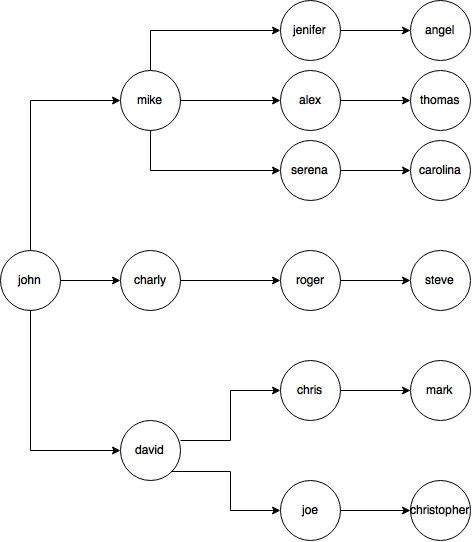
\includegraphics[width=12.5cm,height=9cm]{graph}
\\ \\To compute the answer sets representing 
the solution, the following command is to be invoked:
\\ \centerline{\texttt{shell\$ dlvhex2 --pythonplugin=extsource.py program.hex}}
where \texttt{program.hex} is \hex-program and \texttt{extsource.py} represents the Python file with 
external source implementation (see Section 5). The output of the \dlvhex{} is as follows:


\begin{tabular}{ l r }
   $\mathit{\{personOfInterest(john), friendOfDegree(john,0,john), }$& \\
   $\mathit{invite(john), friendOfDegree(john,1,mike),}$& \\
   $\mathit{friendOfDegree(john,1,david), friendOfDegree(john,1,charly),}$ & \\
   $\mathit{invite(mike),invite(david),invite(charly)\}}$
 \end{tabular}
\\ \\
Note that order of the atoms and the order of answer sets does not bear any meaning. Single answer set for this problem contain atoms given above. As it is expected, the first atom is $\mathit{personOfInterest(john)}$ 
since $\mathit{john}$ is organizing the party and program should generate sets of the friends who should be invited to the party by him. As we specified in the previous section, we can travel at most 1 edge far from the root node. Considering the graph given above only $\mathit{John, Mike, Charly and David}$ are found since they are one edge far from the root node. The next three atoms express who are the new friends discovered and at which depth 
level. For the invitations, it is specified by using aggregates that answer set must have four distinct $\mathit{invites}$ atoms.
In single answer set we have four $\mathit{invites}$ atoms which are $\mathit{invite(john), 
invite(mike), invite(david), invite(charly)}$. Note that this is only answer set possible 
from this program since aggregate constraint is 4 and there are only 4 distinct person that are discovered with depth level 1. 

If we just allow depth level to be larger there may be more answer sets founded due to the fact that more nodes will be discovered. If we decrease minimum number of friends to be invited to the party there may be more than one answer set. Consider that instead of 4 persons we want to invite only 3 persons to the our party. This time we have more than one answer set. Since depth level is still 2 there will be 4 persons discovered again, however out of these 4 persons we have to invite only three of them and one of them will not be invited. According to this we have 4 answer sets in the output of the program. Two of them are showed bellow:\\
\textbf{Answer set 1:}\\
\begin{tabular}{ l r }
   $\mathit{\{personOfInterest(john), friendOfDegree(john,0,john),}$& \\
   $\mathit{invite(john), friendOfDegree(john,1,mike), \mathit{ninvite(charly)},}$& \\
   $\mathit{friendOfDegree(john,1,david), friendOfDegree(john,1,charly),}$ & \\
   $\mathit{invite(mike),invite(david)\}}$
 \end{tabular}
\\ \textbf{Answer set 2:}\\
 \begin{tabular}{ l r }
   $\mathit{\{personOfInterest(john), friendOfDegree(john,0,john),}$& \\
   $\mathit{invite(john), friendOfDegree(john,1,mike), \mathit{ninvite(mike)},}$& \\
   $\mathit{friendOfDegree(john,1,david), friendOfDegree(john,1,charly),}$ & \\
   $\mathit{invite(david),invite(charly)\}}$
 \end{tabular}
\\ \\ This time in answer set we $\mathit{ninvite(charly)} and \mathit{mike}$ since one friend must be discarded and only three will be invited. One can just play with \emph{Depth constraint} and \emph{Aggregate constraint} to see how real output and answer sets will be affected.    


\section{Input Language}% Section No. 3
This section provides an overview of the input language of \dlvhex{} and some examples to illustrate the concepts. 

\subsection{Terms and Atoms}
The vocabulary consists of: terms, constants, variables and external predicates. Terms may be integers, constants, strings and variables as well as the \enquote{\_} tokens. Constant names begin with lowercase letters or are strings enclosed in quotation marks and variable names begin with uppercase letters.

While a constant or string represent itself, a variable is placeholder for all variable-free terms in the language of a logic program. There is a special feature, which is called anonymous variable. The anonymous variable is denoted by ``\_" (the underscore) and is different from a usual variable. Each occurrence of \enquote{\_} represents a new and unique variable, which does not occur anywhere else in the same rule. This might be used to specify that an argument can be ignored or does not matter.

An \emph{atom} has form $\mathit{p(t_1,\dots,t_n)}$ where $p$ is a predicate name, $t_1,\dots,t_n$ are terms and $n$ $\geq$ $0$ is the arity of the predicate atom; a predicate atom $p()$ of arity 0 is likewise represented by its predicate name $p$ without parentheses. Classical atoms are: $q$, $q$ and $-$ $q$.

\begin{exmp}
Terms are:
\\ \text{Constants:} $a$, $1$, $\mathit{a1}$, $\mathit{9862}$, $\mathit{c1}$
\\ \text{Variables:} $X$, $Y$, $Z$
\\ \text{Atoms:} $\mathit{parent}(X,Y)$, $\mathit{employee}(name, salary, ID, location)$
\\ \text{Predicates:} $\mathit{parent}$ $\mathit{employee}$
\end{exmp}
\subsection{Normal Programs and Integrity Constraints}
A \hex{}-program is constructed using \emph{facts, rules and integrity constraints}. 

\begin{center}
\begin{tabular}{ r l r }
\text{Fact:} & \texttt{$A_0$}. & \\
\text{Rule:} & \texttt{$A_0$}& $\leftimpl$  \texttt{$L_1$},\dots, \texttt{$L_n$}. \\
\text{Constraint:}&& $\leftimpl$  \texttt{$L_1$},\dots,\texttt{$L_n$}. 
\end{tabular}
\end{center}
The sign \enquote{$\leftimpl$} is meant to be an implication to the left. The left side of a rule is called its head, and right side is called its body. The head \texttt{$A_0$} of a rule or a fact is an atom of the same syntatic form as a constant or function. In the body of a rule or an integrity constraint, every \texttt{$L_j$} for 1 $\leq$ j $\leq$ n is a literal of the form \texttt{A} or \texttt{not A}, where \texttt{A} is an atom and the connective \texttt{not} denotes default negation. We say that literal L is positive if it is an atom and negative otherwise. While the head atom \texttt{$A_0$} of the fact must unconditionally be true, the intuitive reading of a rule corresponds to an implication: if all positive atoms in the rule body are true and negated atoms are false, then $A_0$ must be true. On the other hand, an integrity constraint is a rule that filters solution candidates, meaning that the literals in its body must not jointly be satisfied. A result of \dlvhex{} computation is called an \emph{answer set} which is a consistent explanation(model) of the world.

\begin{exmp} 
Consider the following logic program:
\begin{align*}
\mathit{ joke }.& \\
\mathit{ laugh } & \leftimpl \mathit{ joke }.
\end{align*} 
\end{exmp}
The first line here represents an \emph{atom} which is always true. The second line is a \emph{rule} and reads as \enquote{If $\mathit{joke}$ is true, $\mathit{laugh}$ must also be true}. Also we can read this as \enquote{from $\mathit{joke}$ follows $\mathit{laugh}$}. The single \emph{model} of above program is $\{\mathit{joke}, \mathit{laugh}\}$ since they are the atoms which are true in the program. To explain the concept of \emph{integrity constraints} we will consider following example:
\begin{exmp}
\begin{align*}
&\mathit{node}(X) \leftimpl \mathit{edge}(X, Y). &\\
&\mathit{node}(Y) \leftimpl \mathit{edge}(X, Y). & \\
&\mathit{colored}(X, r) \vee \mathit{colored}(X, g) \vee \mathit{X, b} \leftimpl \mathit{node}(X). & \\
&\leftimpl \mathit{edge}(X, Y), \mathit(colored)(X, C), \mathit{colored}(Y, C) & \\
&\mathit{edge}(2, 4). \mathit{edge}(2, 3). \mathit{edge}(5, 5). & \\
&\mathit{edge}(4, 6). \mathit{edge}(4, 5). \mathit{edge}(5, 7). & \\
&\mathit{edge}(6, 7). &
\end{align*} 
\end{exmp}
In the first three lines one can see node declarations with variables $X$ and $Y$. We concluded that $X$ and $Y$ are variables since they begin with uppercase letter. It says that: \enquote{If $\mathit{edge}(X,Y)$ is true then $\mathit{node(X)}$ is also true}. That is, it extracts the nodes from a graph specified by its edges. In the \emph{guessing part} all possible node color combinations are generated. Each node may be coloured with either red, green or black. In the checking part, integrity constraint delete all color combinations which does not satisfy the requirement that there may be no edge between two nodes of equal color. 

Another important feature of \dlvhex{} is \emph{default negation}. Negation is treated as ``negation as failure". In other words: if an atom is not true in some model, then its negation should be considered to be true in that model. With this mechanism we can, for example, define the complementary graph of a given graph. This is the graph which has the same nodes, but of all possible edges, it has exactly those edges which do not exist in the original graph.

Note that $\mathit{node}(X)$ and $\mathit{node}(Y)$ need to be included in the body in order to satisfy the following safety requirement for rules: \emph{Variables}, which occur in a negated literal, must also occur in a positive literal in the body.
\begin{exmp}
\begin{align*}
& \mathit{node}(X) \leftimpl \mathit{edge}(X, \_).\\
& \mathit{node}(Y) \leftimpl \mathit{edge}(\_, Y). \\
& \\
& \mathit{comp\_edge}(X, Y) \leftimpl \mathit{node}(X), \mathit{node}(Y), \mathit{not} \text{ } \mathit{edge}(X, Y). 
\end{align*}
\end{exmp}
Here $\mathit{comp\_edge}$ describes the set of edges in the complementary graph. Such an edge must go from one node to another node (possibly the same one), and this edge must not be contained in the original edge set. 

\subsection{Classical Negation}
\dlvhex{} supports two kinds of negation. Here we will emphasize difference between explicitly expressing falseness of an atom and having it done by \emph{Closed World Assumption}. The connective $\mathit{not}$ expresses default negation, i.e. a literal $\mathit{not}$\text{ }$A$ is assumed to hold unless atom $A$ is derived to be true. In contrast, the classical (or strong) negation of an atom holds only if it can be derived. In other words if there is no evidence that an atom is true, it is considered to be false. Classical negation, indicated by symbol \enquote{-}, is permitted in from of an atoms. The semantic relationship between $A$ and $-A$ is simply that they must not jointly hold.

\begin{exmp} 
Imagine a situation where agent has to cross a railroad. The agent should cross it if there is no train approaching. With this description, one might specify the following program:
\begin{align*}
 & \mathit{cross\_railroad} \leftimpl \mathit{not} \text{ } \mathit{train\_approaches}.
\end{align*}
\end{exmp}
The following program has the model \{$\mathit{cross\_railroad}$\} because $\mathit{train\_approaches}$ is assumed to be false (as it being true is not stated anywhere). This kind of negation is called \emph{negation as failure}.
\begin{exmp}
The next program uses so-called true or classical negation. Since $\mathit{- train\_approaches}$ is not known to be true, the following program has only an empty model.
\begin{align*}
\mathit{cross\_railroad} \leftimpl \mathit{- train\_approaches}.
\end{align*}
\end{exmp}
The difference between the two kinds of negation is important: in the first example, the railroad track is crossed if there is no information on any trains approaching, which is quite dangerous, while in the second example, it is only crossed if is is known for sure that no train comes. It is important to note that classical negation is stronger than negation as finite failure.

\subsection{Disjunction}
Disjunctive logic programs permit the connective ``$\vee$" between atoms in rule heads. \\
\begin{center}
\begin{tabular}{ r l l}
  \text{Fact:} & $A_0$ $\vee$ \dots $\vee$ $A_m$ \\
  \text{Rule:} & $A_0$ $\vee$ \dots $\vee$ $A_m$ $\leftimpl$ $L_1,\dots,L_n. $ \\
 \end{tabular}
\end{center}
A \emph{disjunctive head} holds if at least one of its atoms is true. In a simple disjunctive program $\mathit{a} \vee \mathit{b.}$ we have the two answer sets \{$a$\} and \{$b$\}. 

The \emph{head} $A_0$ of a rule or a fact is an atom of the same syntatic form as a constant or function. In the \emph{body} of a rule or an integrity constraint, every $L_j$ for 1 $\leq$ j $\leq$ n is a literal of the form A or $\mathit{not}$ \text{}$A$, where $A$ is an atom and the connective $\mathit{not}$ denotes default negation. We say that literal $L$ is positive if it is an atom and negative otherwise. 
\begin{exmp}
\begin{align*}
& \mathit{left\_arm\_broken} \text{ v } \mathit{right\_arm\_broken}.\\
& \mathit{can\_write} \leftimpl \mathit{left\_arm\_broken}.\\
& \mathit{be\_angry} \leftimpl \mathit{can\_write}.
\end{align*}
\end{exmp}
Suppose we met a friend recently and know that he had one of his arms broken, but do not know which one. Now suppose we did not receive a greeting card for your birthday and wonder if you should be angry on him or he just could not write because his right hand is broken. In the example, \dlvhex{} will generate two possible explanations. The first rule is called a disjunctive rule which is read as \enquote{For sure, either the left or the right arm is broken.} Without being sure which arm is broken \dlvhex{} will evaluate the program and produce the two models $\mathit{\{left\_arm\_broken, can\_write, be\_angry\}}$ and $\mathit{\{right\_arm\_broken\}}$.  

\subsection{Built-in Arithmetic Functions}
Besides integers (constant arithmetic functions), written as sequence of digits $0$,\dots,$9$, \dlvhex{} supports other types of arithmetic functions. We are using the following operators for those functions: $+$ (addition), $-$ (subtraction), $*$ (multiplication), $/$ (integer division). 
\begin{exmp}
\begin{align*}
& \mathit{a}(6). \\
& \mathit{b}(2). \\
& c(X,Y,XX) \text{ } \leftimpl \text{ } a(X), b(Y),+(X, Y, XX). \\
& d(X,Y,XX) \text{ } \leftimpl \text{ } a(X), b(Y),-(X, Y, XX). \\
& e(X,Y,XX) \text{ } \leftimpl \text{ } a(X), b(Y),*(X, Y, XX). \\
& f(X,Y,XX) \text{ } \leftimpl \text{ } a(X), b(Y),/(X, Y, XX).
\end{align*}
\end{exmp}
The single answer set for the example above is:\\ \centerline{$\mathit{\{a(6),b(2),e(6,2,12),f(6,2,3),c(6,2,8),d(6,2,4)\}}$.}
\\Alternatively to \emph{prefix notation} one can also use \emph{infix notation} to use built-in arithmetic functions in \dlvhex{}. For instance $\mathit{+(X, Y, XX)}$ alternatively can be written as $\mathit{XX=X+Y}$. 

\subsection{Built-in Comparison Predicates}
\dlvhex{} feature a total order among variable-free terms using built-in predicates $==$ (equal), $\neq$ (not equal), $<$ (less than), $\leq$ (less than or equal), $>$ (greater than) and $\geq$ (greater than or equal). All kinds of constants (symbols and integers) may be compared against each other freely. If two integers are compared, the semantics is according to numeric values. All other comparisons are just guaranteed to impose a fixed ordering over all constants. The application of comparison literals to integers is illustrated by the following example.
\begin{exmp}
\begin{align*}
& a(1). \\
& a(2). \\
& b(1). \\
& \\
& c(X,Y) \text{ } \leftimpl \text{ } a(X), b(Y), X <> Y. \\
& d(X,Y) :- a(X), b(Y), X \neq Y. \\
& e(X,Y) :- a(X), b(Y), X < Y. \\
& f(X,Y) :- a(X), b(Y), X > Y. \\
& g(X,Y) :- a(X), b(Y), X \leq Y. \\
& h(X,Y) :- a(X), b(Y), X \geq Y. \\
& i(X,Y) :- a(X), b(Y), Y == 1. 
\end{align*}
\end{exmp}
The single answer set for the example above is:\\ $\mathit{\{a(1),a(2),b(1),i(1,1),i(2,1),c(2,1),d(2,1),f(2,1),g(1,1),h(1,1)},$\\
$\mathit{h(2,1)}\}$

\subsection{Conditions and Conditional Literals}
A \emph{conditional literal} is of the form \\ \centerline{$L_0:L_1,\dots,L_n$} where every $\mathit{L_j \text{ } for \text{ } 0 \leq j \leq n}$ is a literal, $L_1,\dots,L_n$ is called \emph{condition}, and \enquote{:} resembles mathematical set notation. Whenever $\mathit{n = 0}$, it is a regular literal and we denote it usually by $L_0$.

For example, the rule $\mathit{a \leftimpl b : c.}$ yields $a$ whenever either $c$ is false (whether $b$ holds or not) or both $b$ and $c$ are true \cite{pott}.

Together  with variables, conditions allow for specifying collections of expressions within a single rule or aggregate. This is particularly useful for encoding conjunctions (or disjunctions) over arbitrarily many ground atoms as well as for the compact representation of aggregates. 
\begin{exmp}
\begin{align*}
& \mathit{person}(\mathit{jane}). \text{ } \mathit{person}(\mathit{john}).\\
& \mathit{day}(\mathit{mon}). \text{ } \mathit{day}(\mathit{tue}). \text{ } \mathit{day}(\mathit{wed}). \text{ } \mathit{day}(\mathit{thu}). \text{ } \mathit{day}(\mathit{fri}). \text{ }\\
& \mathit{available}(\mathit{jane}) \text{ } \leftimpl \text{ } not \text{ } \mathit{on}(\mathit{fri}).\\
& \mathit{available}(\mathit{john})\text{ } \leftimpl \text{ } \mathit{not} \text{ } \mathit{on}(\mathit{mon}), \mathit{not}  \text{ } \mathit{on}(\mathit{wed}).\\
& \mathit{meet} \text{ } \leftimpl \text{ } \mathit{available}(X) : \mathit{person}(X).\\
& \mathit{on}(X) : \mathit{day}(X) \text{ } \leftimpl \text{ } \mathit{meet}.
\end{align*}
\end{exmp}  
We have used the conditions in last two lines of the code. The \emph{conjunction} in the body of line 5 is obtained by replacing $X$ in $\mathit{available(X)}$ with all ground terms $t$ such that $\mathit{person(t)}$ holds, namely, with $\mathit{t=jane}$ and $\mathit{t=john}$. The condition for the last line is contained in the head of the rule. It turns into \emph{disjunction} over all ground instances of $\mathit{on(X)}$ such that $X$ is substituted by terms $t$ for which $\mathit{day(t)}$ holds. Any variable occurring within a condition does not count as a positive occurrence outside the condition in the sense of safety. A variable $X$ in an aggregate-free rule is safe if at least one of the following conditions is satisfied:
\begin{itemize}
\item $X$ occurs in a positive standard predicate in the body of the rule;
\item $X$ occurs in a true negated standard predicate in the body of the rule;
\item $X$ occurs in the last argument of an arithmetic predicate $A$ and all other arguments of $A$ are safe.
\end{itemize}
Variables occurring in atoms not subject to any conditions are global. Each variable within an atom in front of a condition must be global or have a positive occurrence on the right hand-side of the condition. During grounding, the instantiation of global variables take precedence over non-global ones, that is, the former are instantiated before the latter. As a consequence, variables that occur globally are substituted by terms before a condition is further evaluated \cite{pott}.    

\subsection{Aggregates}
Aggregates allow to express properties over set of elements. \hex{}-programs with aggregates often allow clean and concise problem encodings by minimizing the use of auxiliary predicates and recursive programs, and help the programmers to depict problems in a more natural way. For instance, we may state that the sum of a semester's course credits must be at least 20, or that the sum of shopping items must not exceed 30 Euros. We can say that an aggregate is a function on a set of tuples that are normally subject to conditions. By comparing an aggregated value with given values, we can extract a truth value from an aggregate's evaluation, thus obtaining an aggregate atom. They can occur in the bodies of rule and constraints, possibly negated using negation-as-failure \cite{pott}.

The form of an \emph{aggregate atom} occuring in a rule body is as follows:\\ \centerline{$s_1 \prec_1 \alpha \{ t_1:L_1;...;t_n:L_n\} \prec_2 s_2$} 
\\ Here, all $\mathit{t_i}$ and $\mathit{L_i}$, forming \emph{aggregate elements}, are non-empty tuples of terms and literals, respectively. $\alpha$ is the name of some function that is applied to the term tupples \texttt{$t_i$} that remain after evaluating the conditions expressed by $L_i$. Finally,  the result of applying $\alpha$ is compared by means of the comparison predicates $\prec_1 or \prec_2$ to the terms $s_1$ and $s_2$ respectively. $\mathit{\#count}$, $\mathit{\#sum}$, $\mathit{\#times}$, $\mathit{\#min}$, and $\mathit{\#max}$ are called aggregate functions, and \dlvhex{} currently supports exactly these five. An aggregate function is applied over a set and returns a numeric value. Let $f(S)$ be an aggregate function. A variable, X, is a \emph{local variable} to $f(S)$ if and only if $X$ appears in $S$ and $X$ does not appear in any aggregate function that is outer to $f(S)$.
\begin{exmp}
\begin{align*}
& emp(1,goofie,1250).\\
& emp(2,willy,700).\\
& emp(3,woody,750).\\
& emp(4,jerry,900).\\
& emp(5,tom,1050). \\
& over1000(I,S) \leftimpl emp(I,N,S), S > 1000.\\
& over1000nr(X) \leftimpl \#count\{I : over1000(I,W)\} = X, \#int(X).
\end{align*}
\end{exmp}
Intuitively the symbolic set appearing in the aggregate predicate consists of two ground predicates: \\ \centerline{$\{\langle 1 \rangle,\langle 5 \rangle\}$}
\\which are both true w.r.t. the unique model of the whole program, hence \\ \centerline{$ \#count\{over1000(1,1250),over1000(5,1050)\}$} \\returns 2 as output of aggregate function and outputs:\\ \centerline{ $\mathit{emph(1,goofie,1250),emp(2,willy,700),emp(3,woody,750),emp(4,jerry,900),}$}
\\ \centerline{ $\mathit{emp(5,tom,1050),over1000(1,1250),over1000(5,1050),over1000nr(2)}$}
\\as a result of the program.
The aggregate function $\mathit{\#count}$ returns the cardinality of the symbolic set to which it is applied. We want to count how many employees of the company earn more than 1000. 

\bigskip Aggregate function $\mathit{\#sum}$ returns the sum of the first local variable to be aggregated over in the symbolic set. Suppose we want to know how much the Cartoon Co. spends on salaries.
\begin{align*}
\mathit{salaryTotal(X)} \leftimpl \mathit{\#sum}\{S,I : \mathit{emp(I,N,S)}\} = X.
\end{align*}
The symbolic set here consists of 5 elements, namely all of the facts stored in the database of the employees. The aggregate function applied to the given set returns the sum of the salaries of all the employees, the output thus is: \\ \centerline{
\{$\mathit{salaryTotal(4650)}$\}}. $\mathit{\#times}$ is similar to $\mathit{\#sum}$, but computes the product of the first local variable to be aggregated over in the symbolic set. When applied over the empty set, $\mathit{\#times}$ returns 1.
\bigskip \\The aggregate function $\mathit{\#min}$ returns the minimum value of the first local variable to be aggregated over in the symbolic set. The following simple program then returns the lowest income among all employees.
\begin{align*}
& lowest(X) \leftimpl \#min\{S : emp(I,N,S)\} = X.
\end{align*}
The aggregate function applied to the given set returns the minimum salary among of all the employees, the output thus is:
{$\mathit{lowest(700)}$}.
\bigskip \\The aggregate function $\mathit{\#max}$ returns the maximum value of the first local variable to be aggregated over in the symbolic set. The following program computes the maximum income earned in the company
\begin{align*}
& \mathit{highest}(X) \leftimpl \mathit{\#max}\{S : \mathit{emp}(I,N,S)\} = X.
\end{align*}
and it outputs $\{highest(1250)\}$ as a highest income in the company.

\subsection{Optimization}
Introducing \emph{weak constraints} into \hex-programs allows us to formulate several optimization problems in an easy and natural way. These weak constraints are adopted from \emph{DLV}. While standard constraints (integrity constraints, strong constraints) always have to be satisfied, weak constraints should be satisfied if it is possible.


The answer sets of a program P with a set W of weak constraints are those answer sets of P which minimize the violation of weak constraints respecting their weights and levels. They are called best models of (P,W). Note that a program may have several best models.


Weak constraints can be weighted according to their importance (the higher the weight, the more important the constraint). In the presence of weights, best models minimize the sum of the weights of the violated weak constraints. Weak constraints can also be prioritized. Under prioritization, the semantics minimizes the violation of the constraints of the highest priority level first; then the lower priority levels are considered one after the other in descending order. Syntactically, weak constraints are specified as follows. \\ \centerline{:$\mathit{Conj}. [\mathit{Weight}:\mathit{Level}]$} \\ where $\mathit{Conj}$ is a conjunction of (possibly negated) literals, and both $\mathit{Weight}$ and $\mathit{Level}$ are positive integers. Weights and priority levels are allowed to be variables, provided that these variables also appear in a positive literal in $\mathit{Conj}$.
The following program, computes the minimum spanning trees of a weighed directed graph.
\begin{exmp}
\begin{align*}
r_1\colon& \mathit{root}(a). \\
r_2\colon& \mathit{node}(a). \mathit{node}(b). \mathit{node}(c). \mathit{node}(d). \mathit{node}(e). \\
r_3\colon& \mathit{edge}(a,b,4). \mathit{edge}(a,c,3). \mathit{edge}(c,b,2). \mathit{edge}(c,d,3). \\
r_4\colon& \mathit{edge}(b,e,4). \mathit{edge}(d,e,5). \\
r_5\colon& \\
r_6 \colon & \mathit{in\_tree}(X,Y,C) \vee \mathit{out\_tree}(X,Y) \leftimpl \mathit{edge}(X,Y,C), \mathit{reached}(X). \\
r_7\colon& \leftimpl \mathit{root}(X), \mathit{in\_tree}(\_,X,C).\\
r_8\colon& \leftimpl \mathit{in\_tree}(X,Y,C), \mathit{in\_tree}(Z,Y,C), X \neq Z. \\
r_9\colon&  \\
r_{10}\colon& \mathit{reached}(X) \leftimpl \mathit{root}(X). \\
r_{11}\colon& \mathit{reached}(Y) \leftimpl \mathit{reached}(X), \mathit{in\_tree}(X,Y,C). \\
r_{12}\colon& \leftimpl \mathit{node}(X), \mathit{not} \text{ } \mathit{reached}(X). \\
r_{13}\colon&   \\
r_{14}\colon&\mathit{ \sim in\_tree}(X,Y,C). [C:1]
\end{align*}
\end{exmp}
Best model: $\mathit{\{reached(a), out\_tree(a,b), in\_tree(a,c,3), reached(b), reached(c),}\\ \mathit{ in\_tree(b,e,4), in\_tree(c,b,2), in\_tree(c,d,3), reached(e), reached(d),} \\ \mathit{  out\_tree(d,e)\}}$
\\Cost ([Weight:Level]): $<[12:1]>$

Fact from the $r_1$ of the example above defines root node of a tree. Nodes and edges are defined in $r_2$ and $r_3$. Rule from the $r_6$ determines is an edge going from node $X$ (node $X$ is already reached) in the minimum spanning tree or out of it. Integrity constraint from $r_7$ ensures that there is no incoming edges to the root node. $r_8$ eliminates all answer sets where there are two outgoing edges going to same node $Y$. In the $r_{10}$ and $r_{11}$ we have rules that are deciding is node reached or not. $r_{11}$ removes all answer sets where there is any node which is not discovered. Last line of the program is weak constraint with weight $C$ and level 1. Weak constraint should be satisfied, but their violation does not kill the model. Aim is to minimize number of violated weak constraints. In our best model there is no weak constraint which is not satisfied and cost is 12.  


Finally, we show an example where both weights and priorities are specified. This example and some others are taken from the DLV-User Manual \cite{dlvum}. Consider the problem of assigning a given set of employees to two projects. As a minor desideratum, we wish that members of the same group already know each other. Higher level constraints ask each group to be heterogeneous as far as skills are concerned, and require that people married with one another do not work in the same group.
\begin{exmp}
\begin{align*}
r_1\colon& \mathit{employee}(a). \text{ } \mathit{employee}(b). \text{ }  \mathit{employee}(c). \text{ } \mathit{employee(d)}. \\
r_2\colon& \mathit{employee}(e). \\
r_3\colon& \mathit{know}(a,b). \text{ } \mathit{know}(b,c). \text{ } \mathit{know}(c,d). \text{ } \mathit{know}(d,e). \\
r_4\colon& \mathit{same\_skill}(a,b). \\
r_5\colon& \mathit{married(c,d)}. \\
r_6\colon&  \\ 
r_7\colon& \mathit{member}(X,p1) \vee \mathit{member}(X,p2) \leftimpl \mathit{employee}(X).\\
r_8\colon& : \sim \mathit{member}(X,P), \mathit{member}(Y,P), X \neq Y, \mathit{not} \text{ } \mathit{know(X,Y)}. \colon& [1:1] \\
r_{9}\colon& : \sim  \mathit{member}(X,P), \mathit{member}(Y,P), X \neq Y, \mathit{marrie}d(X,Y). & [1:2]\\
r_{10}\colon& : \sim member(X,P), member(Y,P), X \neq Y, same\_skill(X,Y). & [1:2] 
\end{align*}
\end{exmp}
This program has two best models:
\\ \{$\mathit{member}(a,p2), \mathit{member}(b,p1), \mathit{member}(c,p1), \mathit{member}(d,p2), \mathit{member}(e,p2)$\}
\\$\mathit{Cost}$ ($[ \mathit{Weight:Level]}$): $ \langle [6:1],[0:2] \rangle $
\\ \{$\mathit{member}(a,p1), \mathit{member}(b,p2), \mathit{member}(c,p2), \mathit{member}(d,p1), \mathit{member}(e,p1)$\}
\\$\mathit{Cost}$ ($[ \mathit{Weight:Level]}$): $ \langle [6:1],[0:2] \rangle $ '\\

In the $r_1$ and $r_2$ we defined employees as a set of the facts. Rows $r_3$, $r_4$ and $r_5$ specify $\mathit{know}$, $\mathit{same\_skill}$ and $\mathit{married}$ relations between some of employees. Since $\mathit{employee}(X)$ is true, each $\mathit{employee}$ will be assigned either to the project 1 or project 2 what is given in $r_7$. Last three lines of program are weak constraints, this time with same weights but different levels of priority. Under prioritization, the \dlvhex{} minimizes the violation of the constraints of the highest priority level first; then the lower priority levels are considered one after the other in descending order. This time we have two best models in our solution.     


\subsection{Higher-order Atoms}
Now we introduce the most specific feature of \dlvhex{} compared to other ASP solvers. \hex{}-programs are nonmonotonic logic programs admitting \emph{high-order atoms}, and we extend the well known answer-set semantics to this class of programs.

Let $C$,$X$, and $G$ be mutually disjoint sets whose elements are called \texttt{constant names, variable names,} and \texttt{external predicate names,} respectively. Unless explicitly specified, elements from \texttt{$X$} are denoted with first letter in upper case, while elements from \texttt{$G$} are prefixe with \enquote{\&}. 
We note that the constant names serve both as individual and predicate names. Elements from \texttt{$C$} $\cup$ \texttt{$X$} are called \texttt{terms}. \\ \\A high-order atom allows to quantify values over predicate names, and to freely exchange predicate symbols with constant symbols, like in the rule\\ \centerline{\\$C(X) \leftarrow \textit{subclassOf(D,C),D(X)}$}
A \textit{high-order atom} is a tuple ($Y_0, Y_1,\dots,Y_n$), where $Y_0, Y_1,\dots,Y_n$ are terms; $ n \ge 0$ is the \textit{arity} of the atom. Intuiitively, $Y_0$ is the predicate name, and we thus also use the more familiar notation $Y_0(Y_1,\dots,Y_n)$. The atom is \textit{ordinary}, if $Y_0$ is a constant. For example, \textit{(x,rdf:type,c),node(X), and D(a,b),} are atoms;the first two are ordinary atoms. To understand concept better we are providing example which show how we can get use of external atoms in ordinary ASP.

\subsection{External Atoms}
Through external atoms, \hex{}-programs can communicate with other sources of computation; this can be used to model extensions of ASP.  
An \emph{external atom} facilitates to determine the truth value of an atom through an external source of computation.
An \emph{external atom} is of the form \\ \centerline{ \&g[$Y_1,\dots,Y_n$]($X_1,\dots,X_m$),} \\where $Y_1,\dots,Y_n$ and $X_1,\dots,X_m$ are the two lists of terms (called \textit{input} and \textit{output} lists, respectively), and \&g $\in$ \textit{G} is an external predicate name. We assume that \&g has fixed lengths \texttt{in($\&g$)} = n and \texttt{out($\&g$)} = m for input and output lists, respectively. Intuitively, an external atom provides a way for deciding the truth value of an output tuple depending on the extension of a set of input predicates.
For instance, the rule \\ \centerline{ \textit{$reached(X) \leftarrow \&reach[edge,a](X)$}}
\\computes the predicate \textit{reached} taking values from the predicate $\&reach$, which computes via \textit{$\&reach[edge,a](X)$} all the reachable nodes in the graph in the graph \textit{edge} from node \textit{a}, delegating this task to an external computational source.
\begin{exmp}
\begin{align*}
& \mathit{systems}(\mathit{dlvhex}). \mathit{systems}(\mathit{clasp}). \\  
& \mathit{sayhello(X)} \leftimpl \ext{\mathit{concat}}{\mathit{hello, Y}}{\mathit{X}}, \mathit{systems(Y).}  \\ 
& \mathit{set1}(a). \text{ } \mathit{set1}(b). \text{ } \mathit{set1}(c).\\
& \mathit{set2}(b). \text{ } \mathit{set2}(c). \text{ } \mathit{set2}(d).\\
& \mathit{set3}(X) \leftimpl \ext{\mathit{setdiff}}{\mathit{set1, set2}}{\mathit{X}}. 
&
\end{align*}
\end{exmp}

There are two different external sources in this program, first one is $\mathit{\&concatenate}$ and second one is $\mathit{\&setdiff}$. First part of the program for each system concatenates the string \enquote{hello} and a system name using $\mathit{\&concat}$ external source. At output we have the answer set like:\\ 
\centerline{ \{ $\mathit{sayhello}(\mathit{hellodlvhex}), \mathit{sayhello}(\mathit{helloclasp})$ \}}
\\In this case $\mathit{concat}$ external source receives constant input parameters and passes them as a \emph{tuple}. It starts with an empty string and concatenate all constants from input sequence to the one string. The final string is returned as output of the external source.   


Second part of the program works with externals source which has predicate input parameters. $\mathit{setdiff}$ has two predicate input parameters. It is important to notice that there is difference between inputs for the $\mathit{concat}$ and $\mathit{setdiff}$ external sources. $\mathit{concat}$ have constant inputs stored in tuple while $\mathit{setdiff}$ has predicates. Second part of the program first defines two different sets and then computes $\mathit{set1}$ minus $\mathit{set2}$ using $\mathit{\&setdiff}$ external source. At the output we have: $\mathit{set3}(a)$ 




\newpage
\section{References}
\begin{thebibliography}{1}
\bibitem{extatoms} Thomas Eiter, Micheal Fink, Thomas Krennwallner, Christoph Redl {\em Conflict-driven ASP Solving with External Sources} 2003   
  
\bibitem{ref} Francesco Calimeri, Wolfgang Faber, Martin Gebser, Giovambattista Ianni, Roland Kaminski, Thomas Krennwallner, Nicola leone, Francesco Ricca, Torsten Schaub {\em ASP-Core-2 Input Language} 2013.

\bibitem{licnc} GNU Lesser General Public License. Free Software Foundation, Inc. https://www.gnu.org/copyleft/lesser.html 

\bibitem{onlinedemo}dlvhex. Vienna University of Technology. http://www.kr.tuwien.ac.at/research/systems/dlvhex/demo.php 

\bibitem{git}Software for HEX-Programs. GitHub. https://github.com/hexhex/ 

\bibitem{sourceforge}DLVHEX solver for HEX-programs-  Browse Files at SourceForge.net. Sourceforge.net. http://sourceforge.net/projects/dlvhex/files/

\bibitem{prebuilt}KBS-ASP systems. Thomas Krenwallner. http://www.kr.tuwien.ac.at/staff/tkren/deb.html

\bibitem{boost}Boost C++ Libraries. Boost.org. http://www.boost.org/

\bibitem{hexhex}dlvhex. GitHub. https://github.com/hexhex/core

\bibitem{script}Web location for script

\bibitem{extatoms2}Thomas Eiter, Giovamattista Ianni, Roman Schindlauer and hans Tompits {\em A Uniform Integration of Higher-Order Reasoning and External Evaluations in Answer-Set Programming} 


\bibitem{pott}Martin Gebser, Roland Kaminski, Benjamin Kaufmann, Marius Lindauer, Max Ostrowski, Javier Romero, Trosten Schaub and Sven Thiele {\em Pottasco User Guide}

\bibitem{dlvum}Robert Bihlmeyer, Wolfgang Faber, Giuseppe Ielpa, Vincezino Lio and Gerald Pfeifer {\em DLV-User Manual} 
      
 
 \end{thebibliography} 



\end{document}

